% =====================================================================================
\section{Method}
\label{sec:method}

\paragraph{Overview.} A frozen pretrained language model learns $T$ tasks one after another. Each
task gets its own small low-rank adapter, and an adapter is never changed after its task has been
learned. At test time the model is not told which task an input belongs to. A \emph{switch} sends
every input to one task, and the input is answered by the model as it was when that task was
learned. An answer can then change only if the switch changes its route (Lemma~\ref{lem:route}),
so everything that can be said about forgetting is a statement about the rule that sets the route.
We call the whole system FK-LoRA, after the rule \emph{finders keepers}.
This section gives three rules (the first with a variant). The first, and the one we recommend, reads no instruction: \recog{}, a
\emph{recogniser} over all tasks on frozen states of the model itself, which blocks no task, with
an audit of the changed answers from held-out inputs and, in its variant \handicap{}, a bound in advance on what a later task
can take (Section~\ref{sec:audit}). The second, \cert{}, applies when every input carries the instruction of
its task: each task owns a \emph{protected zone} around the frozen word-vectors of its instruction,
an input inside a zone belongs to the oldest task that claims it, and its answer can never change
again; the system returns a certificate with the answer
(Sections~\ref{sec:features}--\ref{sec:guarantee}). The third builds such zones from the inputs of a
task instead of its instruction; its bound does not grow with the number of later tasks, but in our
tests it blocked later tasks (Section~\ref{sec:bound}). Figure~\ref{fig:overview} sets this beside one shared adapter and beside the two published methods we ran, and Figure~\ref{fig:switch} shows the three rules.

\begin{figure}[t]
  \centering
  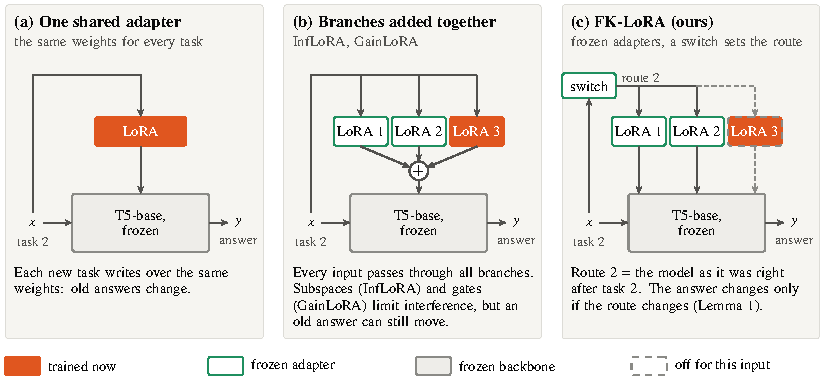
\includegraphics[width=\linewidth]{figures/overview}
  \caption{Three ways to add a task, shown while task~3 is being learned and an input of task~2 is
  answered. (a)~One shared adapter is trained again for each task, so old answers change.
  (b)~InfLoRA and GainLoRA add one branch per task, and every input passes through all branches
  (weighted by gates in GainLoRA); a chosen subspace or the gates limit what a new branch does to
  old inputs, but an old answer can still change. (c)~FK-LoRA never changes an adapter after its
  task has been learned, and a switch sets the route of each input: route~2 is the model as it was
  right after task~2, so the answer changes only if the route changes (Lemma~\ref{lem:route}).}
  \label{fig:overview}
\end{figure}


\subsection{Setting: adapters, routes and answers}
\label{sec:setting}

Let $\mathcal{V}$ be the vocabulary and $E \in \R^{|\mathcal{V}| \times d}$ the input embedding
table of the base model; $E$ and all other base weights $\theta_0$ are frozen. An input is a
sequence of tokens $x = (x_1, \dots, x_L)$.

Task $k$ adds a LoRA adapter \citep{hu2022lora} to every adapted weight matrix $W_0$ of the base
model, $\Delta W_k = \tfrac{\alpha}{r} B_k A_k$ with rank $r$. After $T$ tasks an adapted layer
computes
\begin{equation}
  h \;=\; \Bigl( W_0 + \sum_{k=1}^{T} g_k(x)\, \Delta W_k \Bigr) z ,
  \qquad g_k(x) \in \{0, 1\},
  \label{eq:layer}
\end{equation}
where $z$ is the input of the layer and $g_k(x)$ switches adapter $k$ on or off for the whole input
$x$, in every adapted layer. The methods of this paper differ only in the switches $g_k$. All of
them use a \emph{route} $\rho_T(x) \in \{1, \dots, T\}$ and set
\begin{equation}
  g_k(x) \;=\; \mathbf{1}\bigl[\, k \le \rho_T(x) \,\bigr] ,
  \label{eq:gates}
\end{equation}
so an input with route $j$ is processed by the base model with the adapters of tasks $1, \dots, j$,
which is the model as it was right after task $j$ had been learned. We write
\begin{equation}
  y_T(x) \;=\; F\bigl(x;\; \theta_0,\; \{A_k, B_k\}_{k \le \rho_T(x)}\bigr)
  \label{eq:answer}
\end{equation}
for the answer after $T$ tasks, where $F$ runs the model with a deterministic decoding rule (greedy
decoding in all our experiments).

\begin{lemma}[An answer changes only with its route]
\label{lem:route}
Assume that the adapters of a task are never changed after the task has been learned, that the
base model, its tokenizer, the input template and truncation are fixed, and that decoding is
deterministic. Then for every rule that sets the route, every input $x$ and all times $T' > T$:
if $\rho_{T'}(x) = \rho_T(x)$, then $y_{T'}(x) = y_T(x)$.
\end{lemma}

\begin{proof}
Let $j = \rho_T(x) = \rho_{T'}(x)$, so $j \le T$. By Eq.~\eqref{eq:answer} both answers are
$F(x; \theta_0, \{A_k, B_k\}_{k \le j})$. The adapters of the tasks $1, \dots, j$ exist at time $T$
and are the same at time $T'$, and $F$ is deterministic.
\end{proof}

The lemma uses nothing about the model except that it is a deterministic function of its input and
of the adapters that are switched on. It turns retention into a property of the route: a rule under
which the route of an input cannot change keeps its answer for ever, and a rule under which few
routes change keeps all other answers. The rest of this section is about such rules.

\begin{figure}[t]
  \centering
  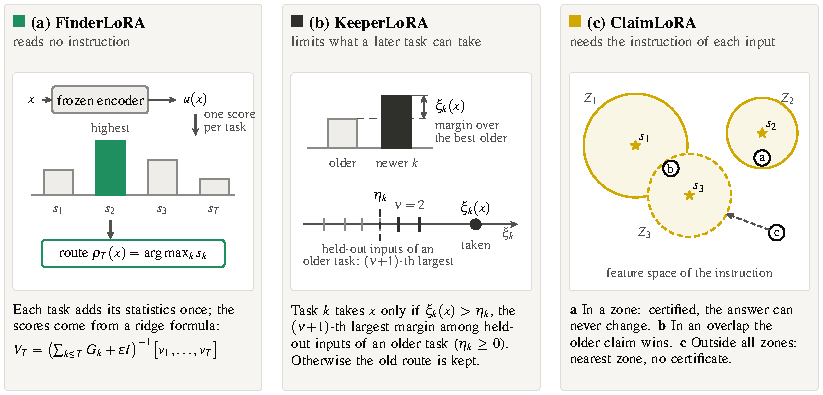
\includegraphics[width=\linewidth]{figures/switch}
  \caption{The three rules that set the route. (a)~\recog{} reads no instruction: it scores every
  task on a frozen feature $u(x)$ of the input with one ridge formula and takes the highest score.
  (b)~\handicap{} adds a handicap for a new task: task $k$ takes an input only if its margin
  $\xi_k(x)$ over the best older task is above $\eta_k$, the $(\nu+1)$-th largest margin among the
  held-out inputs of an older task ($\nu = 2$ in our runs). (c)~\cert{} needs the instruction of
  each input: a task owns a protected zone around the signature of its instruction; an input in a
  zone is certified and belongs to the oldest zone that contains it, and an input outside every
  zone goes to the nearest zone without a certificate.}
  \label{fig:switch}
\end{figure}


% =====================================================================================
\subsection{Without instructions: a recogniser, an audit, and a handicap}
\label{sec:audit}

The rule of this subsection reads no instruction. One classifier over all tasks decides the route
from a frozen feature of the whole input, so no task can be blocked and nothing has to be known
about how a task is worded. Its guarantees are of two kinds: (a) an \emph{audit}, an estimate and a
confidence bound, from held-out inputs, of the share of a task's answers that have changed, valid
for any recogniser that is fitted without those inputs; and (b) a \emph{handicap}, a limit, known
in advance, on what a single later task can take from an older one. The audit is ordinary held-out
estimation, and the handicap is a conformal rank argument with a union bound. What is new is only
this: by Lemma~\ref{lem:route}, both become statements about answers. We first state what no method without instructions can avoid.

\paragraph{The price of having no instruction.} Let two tasks $j < k$ have inputs with
probabilities $p_j(x)$ and $p_k(x)$ (inputs are texts, so there are countably many), and let
$\omega_i(x, y) \in [0, M]$ be the expected score of the answer $y$ to the input $x$ under task
$i \in \{j, k\}$, the expectation being over the reference answers of that task for $x$. Write
$\omega_i^*(x) = \sup_y \omega_i(x, y)$, and for a system that answers $y_T(x)$ at time $T$ let
$\ell_i(T) = \mathbb{E}_{X \sim p_i}\bigl[\omega_i^*(X) - \omega_i(X, y_T(X))\bigr]$ be what it loses on task
$i$ against the best possible answers.

\begin{proposition}[The price of having no instruction]
\label{prop:noinstructionprice}
For every system whose answer at time $T \ge k$, or the distribution of its answer if it answers at
random, depends on the input alone,
\[
  \ell_j(T) + \ell_k(T) \;\ge\; \Omega_{jk} \;:=\; \sum_x \min\bigl(p_j(x), p_k(x)\bigr)\, \gamma_{jk}(x),
\]
where
\[
  \gamma_{jk}(x) \;=\; \inf_y \Bigl[ \bigl(\omega_j^*(x) - \omega_j(x, y)\bigr) + \bigl(\omega_k^*(x) - \omega_k(x, y)\bigr) \Bigr] .
\]
\end{proposition}

\begin{proof}
Fix $x$, let $y = y_T(x)$, $a = \omega_j^*(x) - \omega_j(x, y) \ge 0$ and $b = \omega_k^*(x) - \omega_k(x, y) \ge 0$.
Then $p_j(x)\, a + p_k(x)\, b \ge \min(p_j(x), p_k(x))\,(a + b) \ge \min(p_j(x), p_k(x))\, \gamma_{jk}(x)$.
Sum over $x$. For a system that answers at random, $a$ and $b$ are averages over its answers, each
answer satisfies $a + b \ge \gamma_{jk}(x)$, and the same lines hold.
\end{proof}

Three things follow. (i) If no input belongs to both tasks, $\Omega_{jk} = 0$ and nothing is
forced. This is the case when every input begins with the instruction of its task and no
instruction is the beginning of another: it is the exact sense in which the instruction gives the
task away. (ii) If the score is $M$ for the right answer and $0$ otherwise, and every input that
belongs to both tasks has a right answer under each of them and the two differ, then
$\gamma_{jk} = M$ on those inputs and $\Omega_{jk}/M$ is the overlap of the two input
distributions, one minus their total-variation distance. (iii) The forgetting of task $j$ between
its arrival and time $T$ is $\ell_j(T) - \ell_j(j)$, so
\[
  \bigl(\ell_j(T) - \ell_j(j)\bigr) \;+\; \ell_k(T) \;\ge\; \Omega_{jk} - \ell_j(j) :
\]
what is forgotten of the older task plus what is not learned of the newer one is at least the
conflict $\Omega_{jk}$, minus what the older task never had. A switch with one frozen set of
adapters per task can choose how this sum is split. A rule under which the oldest claim wins
(the zones of Sections~\ref{sec:switch} and~\ref{sec:bound}, below) puts it on the newer task,
except for a share of inputs that is chosen in advance. The recogniser and its variant \handicap{}
put a measured, or a limited, part of it on the older task. Every other method, with shared weights or not, is bound by the same inequality, but
does not say how the sum is split. The proposition is elementary, and that the recognition of the
task limits learning without task labels is known \citep{kim2022theoretical}; we state it because
it gives the recogniser and its variant below their place, and because $\Omega_{jk}$ can be counted from below on a
benchmark (inputs that occur word for word in two tasks; Section~\ref{sec:nodefpublished}).

\paragraph{A joint recogniser.} Let $u(x) \in \mathbb{R}^d$ be a frozen feature of the whole
input (in our experiments the mean of the last-layer states of the frozen encoder of the base
model, without any adapter, standardised with the mean and standard deviation of a fixed pool of
instances of other tasks, Section~\ref{sec:protocol}), and
$\bar u(x) = (u(x), 1)$. When task $k$ arrives, its
training inputs are split at random into fit inputs $D_k^{\mathrm{f}}$ and $m$ held-out inputs
$c_1, \dots, c_m$. The fit inputs add one vector to what is stored and one matrix to a sum kept for
all tasks,
\[
  G_k \;=\; \frac{1}{|D_k^{\mathrm{f}}|} \sum_{x \in D_k^{\mathrm{f}}} \bar u(x)\, \bar u(x)^{\!\top}, \qquad
  v_k \;=\; \frac{1}{|D_k^{\mathrm{f}}|} \sum_{x \in D_k^{\mathrm{f}}} \bar u(x),
\]
so that every task has the same weight, and the recogniser after $T$ tasks is
\begin{equation}
  V_T \;=\; \Bigl(\, \sum_{k \le T} G_k + \varepsilon\, I \Bigr)^{-1} \bigl[\, v_1, \dots, v_T \,\bigr]
  \label{eq:recogniser}
\end{equation}
with a fixed $\varepsilon > 0$. After $T$ tasks the route
of an input is the task with the largest score, the older task in a tie,
\begin{equation}
  \rho_T(x) \;=\; \arg\max_{k \le T}\ \bigl(\bar u(x)^{\!\top} V_T\bigr)_k ,
  \label{eq:jointroute}
\end{equation}
and the answer is given as before by Eq.~\eqref{eq:answer}, with the adapters that existed when
task $\rho_T(x)$ was learned. $V_T$ is the ridge regression of the task labels on the features of
all tasks seen so far. Because the sums are only added, it is the same for every order of
arrival, no input has to be kept, and every task has a column of its own: no task is blocked. The
adapter of a task may be trained on all of its inputs, the held-out ones included; the recogniser
never sees those. A recogniser of this kind is known from class-incremental learning on frozen
features \citep{mcdonnell2023ranpac,zhuang2022acil}; what we add is what is said about its routes.

By Lemma~\ref{lem:route} an answer can change only if its route changes, for this rule as for
any other.

\begin{proposition}[An audit of forgetting from held-out inputs]
\label{prop:audit}
Fix a task $j$ and two times $T' > T \ge j$. Let the fit inputs of all tasks and the choice of the
later tasks be independent of the held-out inputs $c_1, \dots, c_m$ of task $j$ and of a further
input $X$ of task $j$, let the route at every time be fitted without them (as in
Eqs.~\eqref{eq:recogniser}--\eqref{eq:jointroute}), and let $c_1, \dots, c_m, X$ be exchangeable
given everything else. Let $H$ be the number of held-out inputs with
$\rho_{T'}(c_i) \ne \rho_T(c_i)$. Then
\[
  \Pr\bigl[\, y_{T'}(X) \ne y_T(X) \,\bigr] \;\le\; \Pr\bigl[\, \rho_{T'}(X) \ne \rho_T(X) \,\bigr]
  \;=\; \mathbb{E}\Bigl[\frac{H}{m}\Bigr] .
\]
If the inputs are independent draws, then with probability at least $1 - \delta$ over the held-out
inputs, the share of the inputs of task $j$ whose route differs between $T$ and $T'$ is at most
the one-sided Clopper--Pearson upper bound for $H$ successes in $m$ trials at confidence
$1 - \delta$. Both statements also hold when ``differs between $T$ and $T'$'' is replaced by ``is
not the same at all times from $T$ to $T'$'', with $H$ counted in the same way.
\end{proposition}

\begin{proof}
The first inequality holds input by input, as shown above. Let
$I(x) = \mathbf{1}[\rho_{T'}(x) \ne \rho_T(x)]$. Given everything but $c_1, \dots, c_m, X$ the two
routes are fixed functions, so the $m + 1$ numbers $I(c_1), \dots, I(c_m), I(X)$ are exchangeable
and $\Pr[I(X) = 1] = \mathbb{E}[I(c_i)] = \mathbb{E}[H]/m$. For independent draws, $H$ is, given
the routes, binomial with $m$ trials and success probability equal to the share in question, and
the second statement is the definition of the Clopper--Pearson bound. The last sentence follows
with $I(x)$ the indicator that the route of $x$ is not constant from $T$ to $T'$.
\end{proof}

So $H/m$ is an unbiased estimate of the share of changed routes, and the confidence bound is the
guarantee. The condition on independence is not empty: the later tasks may not be chosen by
looking at the held-out inputs, nor at anything computed from them, for example the answers of the
adapters of task $j$, which may have been trained on them. The bound is a statement for one task
and one pair of times. Read at every arrival and for all tasks, the bounds do not hold all at
once at the same confidence; for that the level has to be divided by the number of readings (the
``at all times'' form covers every time in between for one task with a single reading). The audit
needs no pass through the language model: only the features of the held-out inputs are kept. It
can be read before the adapter of a new task is trained, because the recogniser needs only
features: a system knows which older tasks a newcomer disturbs, and by how much, before it learns
the newcomer. The audit says nothing in advance, and it is no longer valid for held-out inputs
that were used to make a decision about the routes. The variant below uses them in exactly this way,
and comes with a bound in advance instead.

\paragraph{A handicap for the newcomer.} When task $k \ge 2$ arrives, compute $V_k$ by
Eq.~\eqref{eq:recogniser} and, for any input, the margin of the newcomer over the best older task,
$\xi_k(x) = (\bar u(x)^{\!\top} V_k)_k - \max_{i < k} (\bar u(x)^{\!\top} V_k)_i$. Fix an integer
$\nu \ge 0$. For each older task $j < k$, take the $(\nu+1)$-th largest value of $\xi_k$ among the
held-out inputs of task $j$ ($-\infty$ if task $j$ has at most $\nu$ of them). Let $\eta_k$ be the
largest of these values, or zero if that is larger. The newcomer \emph{takes} an input if
$\xi_k(x) > \eta_k$. The route is the newest task that took the input:
\begin{equation}
  \rho_T(x) \;=\; \max\bigl\{\, k \le T : \ k = 1 \ \text{ or } \ \xi_k(x) > \eta_k \,\bigr\} .
  \label{eq:handicap}
\end{equation}
The matrices $V_k$ and the thresholds $\eta_k$ are stored when task $k$ arrives and never changed.
So a newcomer takes an input only if the joint recogniser prefers it to every older task, and it
takes at most $\nu$ of the held-out inputs of each older task.

\begin{theorem}[A bound in advance without zones]
\label{thm:handicap}
Let the route be set by Eq.~\eqref{eq:handicap}, under the conditions of
Lemma~\ref{lem:route}. Let $X$ be an input of task $j$ that is exchangeable
with the $m$ held-out inputs $c_1, \dots, c_m$ of task $j$ given everything else, and let the
later tasks and their fit inputs be independent of $(c_1, \dots, c_m, X)$, for example fixed in
advance. If the sequence ends with task $T_{\mathrm{end}}$, then
the probability that the answer to $X$ changes at any time after task $j$ has arrived is at most
the probability that its route does, and
\[
  \Pr\bigl[\ \text{there are } j \le T < T' \le T_{\mathrm{end}} \text{ with } \rho_{T'}(X) \ne \rho_T(X) \ \bigr]
  \;\le\; \frac{(T_{\mathrm{end}} - j)\,(\nu+1)}{m+1} .
\]
\end{theorem}

\begin{proof}
By Eq.~\eqref{eq:handicap} the route of an input changes at the arrival of task $k$ only if the
newcomer takes it, that is, only if $\xi_k(X) > \eta_k$, and it changes at no other time, because
the margins and thresholds of the earlier tasks are frozen. The function $\xi_k$ is fitted on fit
inputs only, so given everything else the $m + 1$ numbers
$\xi_k(c_1), \dots, \xi_k(c_m), \xi_k(X)$ are exchangeable. The threshold $\eta_k$ depends on the
held-out inputs, but all that is used is that it is at least the $(\nu+1)$-th largest of the
first $m$ of these numbers. Among $m + 1$ exchangeable numbers, the last one is strictly larger
than the $(\nu+1)$-th largest of the others with probability at most $(\nu+1)/(m+1)$, ties
included. A union bound over the $T_{\mathrm{end}} - j$ later tasks gives the claim.
\end{proof}

\begin{remark}[What these statements do not say]
\label{rem:auditlimits}
\emph{(i) They bound change, not quality:} an input that the
recogniser gives to the wrong task from the start does not change, and is answered by the wrong
adapters. How many inputs go to their own task is measured, not guaranteed.
\emph{(ii) The price of the handicap is paid by the newcomer} and is seen when it arrives: the
share of its own held-out inputs that it does not take. With $\nu = 0$ one held-out input of an
older task that looks like the newcomer can be enough to keep most of the newcomer out.
\emph{(iii) The bound in advance grows with the number of later tasks and falls with the number of
held-out inputs.} For $m = 200$, $\nu = 2$ and $14$ later tasks it is $21\%$; what we measured on
test inputs was far smaller (Section~\ref{sec:recogniser}), because most later tasks take nothing
from most older ones, which the bound cannot know. A tighter bound in advance needs more held-out
inputs. They are not lost for training: the adapter may learn from them. Under the handicap the
audit of Proposition~\ref{prop:audit} is not valid for the same held-out inputs, because they set
the thresholds; a second held-out set would be needed for both.
\emph{(iv) All statements need test inputs that are like the training inputs of the task}
(exchangeability), and later tasks that were not chosen by looking at the held-out inputs or at
anything computed from them. The probabilities are over the held-out inputs and the test input
together; for one given split the share can be larger (compare
Remark~\ref{rem:boundlimits}(ii)).
\emph{(v) Nothing here reads an instruction.} When inputs do carry one, the feature can be computed
from the example alone while the adapters read the whole input. For a fixed input the answer then
still depends on the route only, and the route does not depend on how the instruction is worded.
So the audit and the bound hold for every wording of the instruction, and also when there is no instruction; the
exchangeability is then a statement about the examples. A system that receives one string has to
find where the example begins; the benchmarks give the two parts separately. A first test with trained answers is in Section~\ref{sec:exampleroutes}.
\end{remark}


\subsection{With instructions: word-vector features of the opening}
\label{sec:features}

The recogniser of Section~\ref{sec:audit} never reads an instruction. When every input does carry
the instruction of its task, a second rule is possible, and it gives an exact statement instead of
a measured one. In instruction tuning every input of task $k$ is built
from a template: the same text, the task's instruction, followed by the instance. We call the part
of the template that comes before the instance the \emph{opening} $o_k$ of the task and write $n_k$
for its length in tokens; we find it as the longest common token prefix of the template filled with two
different instances (Appendix~\ref{app:impl}). An input that begins with it carries the task's
\emph{original wording}, or is \emph{unedited}. The rule of this and the next four subsections looks
at the opening only.

The switch reads an input through weighted averages of its word-vectors. Let $\mathcal{B}$ be a
fixed collection of \emph{unrelated} inputs, taken from tasks that are never learned
(Section~\ref{sec:protocol}), and let $p(v)$ be the share of token $v$ among all tokens of
$\mathcal{B}$. A token counts with the weight
\begin{equation}
  w(v) \;=\; \frac{a}{a + p(v)} , \qquad a = 10^{-3},
  \label{eq:weights}
\end{equation}
so that frequent tokens such as articles and punctuation count little. This is the weighting of
\citet{arora2017simple} for averaged word-vectors, with their usual constant. For a number of
tokens $n$ the \emph{prefix average} of an input is
\begin{equation}
  \varphi_n(x) \;=\; \frac{\sum_{i=1}^{\min(n, L)} w(x_i)\, E_{x_i}}{\sum_{i=1}^{\min(n, L)} w(x_i)} \;\in\; \R^d ,
  \label{eq:prefix}
\end{equation}
and $\varphi_\infty(x)$ is the average over the whole input. Averages are rescaled so that
unrelated inputs vary by about the same amount in every direction. Let $\mu$ and $C$ be the mean
and the covariance matrix of $\{\varphi_{64}(b) : b \in \mathcal{B}\}$ and
\begin{equation}
  \hat{C} \;=\; \tfrac{1}{2}\, C + \tfrac{1}{2}\, \frac{\operatorname{tr} C}{d}\, I ,
  \qquad
  \psi_n(x) \;=\; \hat{C}^{-1/2} \bigl( \varphi_n(x) - \mu \bigr) .
  \label{eq:whiten}
\end{equation}
The shrinkage towards the identity keeps $\hat{C}$ well conditioned. The length 64 is a fixed
choice of the order of a typical opening; these statistics only set a common scale for distances.
All quantities in this subsection depend only on the base model and on $\mathcal{B}$; they are
computed once, before the first task, and never change.

\subsection{Protected zones}
\label{sec:zones}

\begin{definition}[Signature, radius, zone]
When task $k$ is learned, it stores three things. Its \emph{signature} is the feature of its opening,
\begin{equation}
  s_k \;=\; \psi_{n_k}(o_k) \;=\; \psi_{n_k}(x) \quad \text{for every input } x \text{ of task } k \text{ in its original wording}.
  \label{eq:signature}
\end{equation}
Let $\mathcal{S}_k$ be the set of signatures known at that moment: the signatures of the unrelated
tasks from which $\mathcal{B}$ is drawn, computed from their openings in the same way, and
$s_1, \dots, s_{k-1}$. The \emph{radius} of task $k$ is
\begin{equation}
  R_k \;=\; \kappa \cdot \min_{s \in \mathcal{S}_k} \lVert s_k - s \rVert_2 , \qquad \kappa = \tfrac{1}{2} .
  \label{eq:radius}
\end{equation}
The \emph{protected zone} of task $k$ and the \emph{relative distance} of an input from task $k$ are
\begin{equation}
  Z_k \;=\; \{\, x \;:\; \lVert \psi_{n_k}(x) - s_k \rVert_2 \le R_k \,\} ,
  \qquad
  \delta_k(x) \;=\; \frac{\lVert \psi_{n_k}(x) - s_k \rVert_2}{R_k} ,
  \label{eq:zone}
\end{equation}
so that $x \in Z_k$ exactly when $\delta_k(x) \le 1$. If $R_k = 0$, which happens when $s_k$ equals a known signature (for example when the opening
of task $k$ is identical to a known one), we set $\delta_k(x) = 0$ for inputs at distance zero and
$\delta_k(x) = \infty$ for all others.
\end{definition}

The triple $(n_k, s_k, R_k)$ is all that is kept about task $k$ besides its frozen adapter: one
integer, one vector of $d$ numbers and one radius. No example, no statistic of hidden activations
and no trained module is stored. The zone of a task is a ball around its signature whose radius
reaches half-way to the nearest task known when it was created. Zones can overlap: the radius of an older zone
was fixed before newer signatures existed, and each zone measures distance in its own feature $\psi_{n_k}$. An input can
therefore lie in several zones; it then goes to the oldest. An input whose first $n_k$ tokens
are the opening $o_k$ has $\delta_k(x) = 0$ and is in $Z_k$; an input whose instruction was edited
is in $Z_k$ as long as the edit moves the weighted average of its first $n_k$ tokens by at most
$R_k$.

\subsection{The certified switch}
\label{sec:switch}

\begin{definition}[Route and certificate]
After $T$ tasks, the \emph{certificate} of an input and its \emph{route} are
\begin{align}
  c_T(x) &\;=\; \mathbf{1}\bigl[\, x \in Z_1 \cup \dots \cup Z_T \,\bigr] , \label{eq:certificate}\\[2pt]
  \rho_T(x) &\;=\;
  \begin{cases}
    \min \{\, k \le T : x \in Z_k \,\} & \text{if } c_T(x) = 1 \quad \text{(the oldest zone that contains } x \text{)}, \\[2pt]
    \arg\min_{k \le T}\; \delta_k(x) & \text{if } c_T(x) = 0 \quad \text{(the nearest zone)} .
  \end{cases}
  \label{eq:route}
\end{align}
\end{definition}

An input inside a zone is \emph{certified}. An input outside every zone still gets an answer, from
the task whose zone is nearest in units of its own radius, but without a certificate. Whenever two
tasks are equally near, here and in every rule that uses zones or centres, the older one is taken. We call the
rule of Eq.~\eqref{eq:route} \cert{}. A variant of the step for inputs outside every zone, which takes the scale from the unrelated tasks only instead of the radius, is tested in Section~\ref{sec:paraphrase}. Two simpler rules serve as comparisons. \nearest{} uses
$\arg\min_k \delta_k(x)$ for every input and gives older zones no priority. \centre{} gives an input
to the task whose stored centre is nearest to the whole-input feature $\psi_\infty(x)$, where the
centre of a task is the mean of $\psi_\infty$ over its training inputs (with the statistics of
Eq.~\eqref{eq:whiten} computed from whole-input averages); this is the fallback of the first
version of our method, but with the token weights of Eq.~\eqref{eq:weights}; the first version weighted all tokens equally and
behaved differently (Appendix~\ref{app:history}).

\paragraph{Learning a task.} Learning task $t$ takes four steps. (1) Compute $n_t$, $s_t$ and $R_t$
from the task's inputs and store them; from now on $Z_t$ is fixed. (2) Count the training inputs
that lie in an older zone, $b_t = |\{x \in D_t : x \in Z_1 \cup \dots \cup Z_{t-1}\}|$,
and report the number. (3) Add a new adapter $(A_t, B_t)$ with $B_t = 0$ and freeze all older
adapters. (4) Train $(A_t, B_t)$ on the task's data with the usual loss, with the switches of
Eq.~\eqref{eq:gates} in place. Nothing else is added to the loss. A training input of task $t$
has $\delta_t(x) = 0$. If no older zone contains it, its route is $t$ and all adapters are on,
exactly as in plain sequential training of adapters. If an older zone contains it, its route is
smaller than $t$, the new adapter is switched off on it, and it contributes no gradient. We call
such an input \emph{blocked} and say that task $t$ \emph{collides} with the older task.

\paragraph{Answering.} For an input $x$, compute $\psi_{n}(x)$ for the distinct opening lengths
$n \in \{n_1, \dots, n_T\}$, the relative distances $\delta_1(x), \dots, \delta_T(x)$, the route and
the certificate by Eqs.~\eqref{eq:certificate}--\eqref{eq:route}, and run the model once with the
adapters $1, \dots, \rho_T(x)$. Return the answer $y_T(x)$ together with $c_T(x)$. The extra cost is
one lookup in the embedding table, one product with $\hat C^{-1/2}$ per distinct opening length, and $T$ distances in $\R^d$ per input, which is negligible next to
one pass through the model.

Algorithm~\ref{alg:switch} puts the two procedures side by side.

\begin{algorithm}
  \caption{The certified switch}
  \label{alg:switch}
  \small
  \begin{tabular}{@{}r@{\hspace{0.8em}}p{0.92\linewidth}@{}}
    \multicolumn{2}{@{}l}{\textbf{Once}, before the first task (frozen embedding table $E$, unrelated inputs $\mathcal{B}$):} \\[1pt]
    1 & compute the token weights $w$ (Eq.~\ref{eq:weights}), the mean $\mu$ and the rescaling $\hat{C}^{-1/2}$ (Eq.~\ref{eq:whiten}), and the
        signatures of the unrelated tasks \\[4pt]
    \multicolumn{2}{@{}l}{\textbf{Learn task $t$} (training inputs $D_t$; zones and adapters of tasks $1, \dots, t-1$):} \\[1pt]
    2 & $o_t \leftarrow$ the opening of task $t$ (the longest common token prefix of its template filled with two instances); \quad $n_t \leftarrow$ its length in tokens \\
    3 & $s_t \leftarrow \psi_{n_t}(o_t)$; \quad $R_t \leftarrow \kappa \cdot \min_{s \in \mathcal{S}_t} \lVert s_t - s \rVert_2$
        \hfill \emph{the zone $Z_t$ is fixed from here on} \\
    4 & $b_t \leftarrow \bigl|\{x \in D_t : x \in Z_1 \cup \dots \cup Z_{t-1}\}\bigr|$; \quad report $b_t$
        \hfill \emph{blocked inputs} \\
    5 & add adapter $t$ with a zero update; freeze the adapters $1, \dots, t-1$ \\
    6 & train adapter $t$ on $D_t$ with the usual loss; each input $x$ is processed with the adapters $1, \dots, \rho_t(x)$ \\[4pt]
    \multicolumn{2}{@{}l}{\textbf{Answer input $x$} (after $T$ tasks):} \\[1pt]
    7 & $\delta_k \leftarrow \lVert \psi_{n_k}(x) - s_k \rVert_2 \,/\, R_k$ \quad for $k = 1, \dots, T$ \quad (with the convention of Definition~1 if $R_k = 0$) \\
    8 & \textbf{if} some $\delta_k \le 1$: \quad $\rho \leftarrow \min\{k : \delta_k \le 1\}$, \quad $c \leftarrow 1$
        \hfill \emph{the oldest claim wins} \\
    9 & \textbf{else}: \quad $\rho \leftarrow \arg\min_k \delta_k$, \quad $c \leftarrow 0$
        \hfill \emph{nearest zone, no certificate} \\
    10 & \textbf{return} the answer of the base model with the adapters $1, \dots, \rho$, together with $c$ \\
  \end{tabular}
\end{algorithm}

\subsection{What the zones guarantee}
\label{sec:guarantee}

\begin{theorem}[Write-once answers]
\label{thm:writeonce}
Assume that zones and adapters are never changed after they have been created, that the base model, its tokenizer, the input template and truncation, and the quantities of Section~\ref{sec:features} are fixed, and that decoding is deterministic. Let
$x$ be any input with $c_T(x) = 1$. Then for every later time $T' \ge T$ and for every choice of the
tasks $T+1, \dots, T'$,
\[
  c_{T'}(x) = 1, \qquad \rho_{T'}(x) = \rho_T(x), \qquad y_{T'}(x) = y_T(x) .
\]
\end{theorem}

\begin{proof}
Let $j = \rho_T(x) = \min\{k \le T : x \in Z_k\}$. The zones $Z_1, \dots, Z_T$ are the same sets at
time $T'$, because the triples $(n_k, s_k, R_k)$ and the feature map are fixed. Hence
$\{k \le T' : x \in Z_k\} = \{k \le T : x \in Z_k\} \cup \{k : T < k \le T',\ x \in Z_k\}$. The first
set is non-empty with minimum $j \le T$, and every element of the second set is larger than $T$, so
the minimum of the union is $j$. Therefore $c_{T'}(x) = 1$ and $\rho_{T'}(x) = j$. By
Eq.~\eqref{eq:answer} the answer depends on $x$, on $\theta_0$ and on the adapters $1, \dots, j$
only. None of them has changed, and decoding is deterministic, so $y_{T'}(x) = y_T(x)$.
\end{proof}

The proof uses nothing about the model except that it is a deterministic function of its input and
of the weights that are switched on. It does not use the data of later tasks, their number, their
similarity to old tasks or the way their adapters are trained.

\begin{remark}[Other zones]
\label{rem:otherzones}
The proof uses only that $Z_1,\dots,Z_T$ are the same sets at every later time. It therefore applies to any zone whose membership is a
deterministic function of the input, of parts frozen before the first task (another feature, a second model) and of quantities stored when the task arrives
(for example its instruction), and does not depend on any later task, provided that function is computed reproducibly: bit for bit, or with inputs within a fixed tolerance of the border decided by a fixed convention.
A zone decided by a comparison with the instruction has to store the instruction text, not one vector, one radius and one integer.
\end{remark}

\begin{corollary}[Zero forgetting on certified inputs]
\label{cor:zero}
Let $\mathcal{X}$ be a set of inputs that are all certified after $T$ tasks, and let $m$ be any fixed, deterministic score of an
answer against reference answers. Then $\sum_{x \in \mathcal{X}} m(y_{T'}(x)) = \sum_{x \in \mathcal{X}} m(y_T(x))$ for all
$T' \ge T$. In particular, if every test input of task $k$ is certified once task $k$ has been
learned, the forgetting of task $k$ is exactly zero under any such metric and for any later tasks, and
not a single answer changes.
\end{corollary}

\begin{proposition}[The original wording is always certified]
\label{prop:own}
Every input whose first $n_k$ tokens are the opening $o_k$ satisfies $\delta_k(x) = 0$, so it lies in
$Z_k$ and is certified from the moment task $k$ arrives. Its route is $k$ unless an older
zone contains it.
\end{proposition}

\begin{proof}
By Eq.~\eqref{eq:prefix} the prefix average $\varphi_{n_k}(x)$ depends only on the first $n_k$ tokens
of $x$, which are $o_k$. Hence $\psi_{n_k}(x) = s_k$ and $\delta_k(x) = 0 \le 1$.
\end{proof}

The zone also contains inputs whose instruction has been edited, and how far an edit can go
can be bounded without looking at the edit itself. Read the first $n_k$ tokens of an input as a bag
of tokens (if an input has fewer than $n_k$ tokens, its bag is the whole input). For an input $x$ that carries the opening $o_k$ and an arbitrary input $x'$, let $W_{\mathrm{c}}$ be
the total weight, by Eq.~\eqref{eq:weights}, of the tokens that the two bags have in common, $W_{\mathrm{r}}$
the weight of the tokens that only $x$ has (removed by the edit) and $W_{\mathrm{a}}$ the weight of the tokens
that only $x'$ has (added by the edit). Let
\begin{equation}
  \lambda \;=\; \frac{W_{\mathrm{r}}}{W_{\mathrm{c}} + W_{\mathrm{r}}}, \qquad \lambda' \;=\; \frac{W_{\mathrm{a}}}{W_{\mathrm{c}} + W_{\mathrm{a}}}, \qquad
  D \;=\; \max_{u, v \in \mathcal{V}} \bigl\lVert \hat{C}^{-1/2} (E_u - E_v) \bigr\rVert_2 ,
  \label{eq:shares}
\end{equation}
so $\lambda$ and $\lambda'$ are the shares of the weight that the edit removes and adds, and $D$ is
the largest distance between two rows of the rescaled embedding table.

\begin{proposition}[A certified radius for edits]
\label{prop:edits}
Let $R_k > 0$. With the notation of Eq.~\eqref{eq:shares}, $\delta_k(x') \le \max(\lambda, \lambda')\, D / R_k$.
Hence every edit with $\max(\lambda, \lambda') \le R_k / D$ leaves the input inside $Z_k$: it is
certified, and by Theorem~\ref{thm:writeonce} its answer never changes. In particular an input
whose first $n_k$ tokens are a permutation of the opening has $\delta_k = 0$.
\end{proposition}

\begin{proof}
Let $m_{\mathrm{c}}$, $m_{\mathrm{r}}$ and $m_{\mathrm{a}}$ be the weighted means of the embedding rows of the common, the removed
and the added tokens (bags are multisets, so a token that occurs twice counts twice). By
Eq.~\eqref{eq:prefix}, $\varphi_{n_k}(x) = m_{\mathrm{c}} + \lambda\,(m_{\mathrm{r}} - m_{\mathrm{c}})$ and
$\varphi_{n_k}(x') = m_{\mathrm{c}} + \lambda'\,(m_{\mathrm{a}} - m_{\mathrm{c}})$. Assume $\lambda' \ge \lambda$; the other case is
symmetric. Then
\[
  \varphi_{n_k}(x') - \varphi_{n_k}(x) \;=\; \lambda\,(m_{\mathrm{a}} - m_{\mathrm{r}}) \;+\; (\lambda' - \lambda)\,(m_{\mathrm{a}} - m_{\mathrm{c}}) .
\]
Each of $m_{\mathrm{c}}$, $m_{\mathrm{r}}$, $m_{\mathrm{a}}$ is a convex combination of rows of $E$, and the diameter of a set
equals the diameter of its convex hull, so after the linear map $\hat{C}^{-1/2}$ each of the two
differences has norm at most $D$. Hence
$\lVert \psi_{n_k}(x') - s_k \rVert_2 \le \lambda D + (\lambda' - \lambda) D = \lambda' D$. If the bags
have nothing in common, $\lambda = \lambda' = 1$ and the bound is the diameter itself. A
permutation has $W_{\mathrm{r}} = W_{\mathrm{a}} = 0$.
\end{proof}

The bound is a worst case: it has to hold even when the edit exchanges the two most different
tokens of the vocabulary. Section~\ref{sec:edits} compares it with what random edits actually do.
The last sentence of the proposition is also a limit of the method: the switch reads \emph{which}
words open an input, not in which order they come.

\begin{proposition}[The price is paid at admission and is visible]
\label{prop:price}
Let $b_t$ be the number of training inputs of task $t$ that lie in an older zone. These inputs are
routed to an older task now and for ever, whatever adapter $t$ learns, and they contribute no
gradient to adapter $t$. The number $b_t$ is known before task $t$ is trained. If $b_t = 0$ and every training input carries the opening $o_t$ (true in all our runs), training is identical, step for step, to plain sequential
training of adapters.
\end{proposition}

\begin{proof}
For $x$ in an older zone, $\rho_t(x) < t$ by Eq.~\eqref{eq:route}, so $g_t(x) = 0$ in
Eq.~\eqref{eq:gates}: adapter $t$ is multiplied by zero in every layer, in the forward and in the
backward pass, and by Theorem~\ref{thm:writeonce} the route never changes. If $b_t = 0$, every
training input has $\delta_t(x) = 0$ and lies in no older zone, so its route is $t$ and all switches
are one.
\end{proof}

The number $b_t$ is counted on the training inputs. When openings have different lengths, whether
an input of the new task lies inside an older zone can depend on its instance, so $b_t = 0$ does not
exclude that some unseen input of task $t$ lies inside an older zone and stays with the older task.
In the large collection of Section~\ref{sec:many} some tasks had only part of their inputs blocked.

\begin{proposition}[What can still change]
\label{prop:uncertified}
Let $c_T(x) = 0$. When task $T+1$ is added, the route of $x$ changes only if
$\delta_{T+1}(x) < \min_{k \le T} \delta_k(x)$, that is, only if the new task is nearer to $x$, in
relative distance, than every old one. The route of an input never changes after the input has
become certified. An uncertified input can change its route several times as tasks are added.
\end{proposition}

\begin{proof}
The relative distances $\delta_1(x), \dots, \delta_T(x)$ do not change when a task is added, and
they are all larger than one. Ties go to the older task, so the minimiser over $k \le T+1$ differs
from the old one only if $\delta_{T+1}(x)$ is strictly smaller than the old minimum; this covers
the case $x \in Z_{T+1}$, in which the route becomes $T+1$ and Theorem~\ref{thm:writeonce} applies
from then on.
\end{proof}

\begin{remark}[Three consequences that should not be overlooked]
First, the guarantee is about \emph{certified} inputs only; how many inputs are certified is an
empirical question, answered in Section~\ref{sec:results}. Second, the guarantee gives older tasks
priority: a later task whose inputs fall into an older zone cannot be learned on those inputs
(Proposition~\ref{prop:price}). Third, exact retention rules out \emph{backward transfer}: a
certified answer can never get better through later tasks either.
\end{remark}

\begin{remark}[A vanishing radius, and the exact key]
If the radius factor $\kappa$ tends to zero, $Z_k$ shrinks to the inputs whose weighted prefix
average equals the signature, in practice the unedited inputs. All other inputs leave the zones and are routed by $\arg\min_k \delta_k(x)$, which does not depend on $\kappa$ because $\kappa$ cancels;
their routes can therefore differ from those at $\kappa = \tfrac12$, where a certified input goes to the oldest zone that contains it. The limit of \cert{} is therefore
\nearest{} with a certificate for unedited inputs only. The rule we call \keyswitch{} is a different
one: it also matches the opening token for token, but an input that matches no opening gets all
adapters, as in \plain{}. It keeps unedited inputs for ever unless a later task's opening extends theirs, and gives no protection at all to an
input whose instruction has been reworded (Section~\ref{sec:results}). Formally, \keyswitch{} routes $x$ to the task with the
longest opening that $x$ carries token for token (the older one if two are equally long), and to $T$ (all adapters) if there is none.
\end{remark}

\begin{remark}[Exactness in practice]
The route is a deterministic function of the token sequence, computed in 64-bit floating point;
positions that only pad a batch contribute exact zeros. Rounding could in principle decide an
input that lies almost exactly on the border of a zone differently in two runs; we did not observe
this. The theorem speaks about the same adapters being switched on. In the implementation the
adapters of later tasks are multiplied by zero rather than removed, and in every case we compared
the answer was identical, as a string, to the answer given before those tasks existed
(Section~\ref{sec:results}). The theorem is about the function $F$. An implementation computes $F$
in floating-point arithmetic, and its output can depend on how inputs are put into batches and on
hardware and library versions; in one of our runs 6 of 1{,}500 answers of a baseline differed
between batches of 16 and of 32. ``The same answer'' therefore presupposes the same inference
set-up.
\end{remark}

\subsection{A variant for collections with sibling tasks}
\label{sec:exactfirst}

Proposition~\ref{prop:price} names a cost that grows with the number of tasks: a new task whose
instruction resembles an old one lies inside the old zone, and its inputs are blocked.
Section~\ref{sec:many} measures how often this happens in a large collection of real tasks. The
following variant serves such sibling tasks. It was designed after that measurement, and we state
it separately because its guarantee is weaker than Theorem~\ref{thm:writeonce}.

\begin{definition}[Exact claims first]
Let $X_T(x) = \{\, k \le T : \text{the first } n_k \text{ tokens of } x \text{ are } o_k \,\}$ be the
set of tasks whose opening the input carries token for token. The rule \exactfirst{} uses the route
\begin{equation}
  \rho^{\mathrm{x}}_T(x) \;=\;
  \begin{cases}
    \min X_T(x) & \text{if } X_T(x) \neq \emptyset \quad \text{(the oldest exact claim)}, \\[2pt]
    \rho_T(x) & \text{otherwise} \quad \text{(Eq.~\ref{eq:route})} ,
  \end{cases}
  \label{eq:exactfirst}
\end{equation}
and certifies an input if $X_T(x) \neq \emptyset$ or $c_T(x) = 1$.
\end{definition}

The unedited inputs of a new task carry its opening, so their route is the new task even when they
lie inside an older zone. The only task that still cannot be learned is one whose opening is
identical to, or begins with, the opening of an older task. Two things should be kept in mind. A
sibling of an old task is served only word for word: an \emph{edited} input of the sibling that lies
inside the old zone goes to the old task, with a certificate. And the certificate now stands for
two different promises, an unconditional one for exact claims and a conditional one for the other
inputs inside a zone.

\begin{proposition}[What exact claims first guarantees]
\label{prop:exactfirst}
Under the assumptions of Theorem~\ref{thm:writeonce}, with the routes of Eq.~\eqref{eq:exactfirst}:
(i) if $X_T(x) \neq \emptyset$, the route and the answer of $x$ are the same at every later time,
whatever the later tasks are; (ii) if $X_T(x) = \emptyset$ and $c_T(x) = 1$, the route and the answer
of $x$ are the same at every later time $T'$ unless one of the tasks $T+1, \dots, T'$ has an opening
that $x$ carries token for token; (iii) for an input with $X_T(x) = \emptyset$ or
$\min X_T(x) = \rho_T(x)$ the rule gives the route of \cert{}. Since $X_T(x) \subseteq \{k : x \in Z_k\}$, always
$\min X_T(x) \ge \rho_T(x)$; the two rules differ only when an older zone contains an unedited input of a newer task.
\end{proposition}

\begin{proof}
(i) Later tasks have larger indices, so $\min X_{T'}(x) = \min X_T(x)$, and the adapters up to this
route are frozen. (ii) If no later opening is carried by $x$, then $X_{T'}(x) = \emptyset$ and the
route is $\rho_{T'}(x)$, which equals $\rho_T(x)$ by Theorem~\ref{thm:writeonce}. (iii) If $X_T(x)=\emptyset$ the route is $\rho_T(x)$ by Eq.~\eqref{eq:exactfirst}. Every $k\in X_T(x)$ has $\delta_k(x)=0$, so $x\in Z_k$ and $\min X_T(x)\ge\rho_T(x)$; equality gives the route of \cert{}, and strict inequality means that the older zone $Z_{\rho_T(x)}$ contains an unedited input of the newer task $\min X_T(x)$.
\end{proof}

Table~\ref{tab:guarantees} places the three rules that use zones side by side. \cert{} gives the
strongest promise and blocks siblings. \nearest{} serves siblings and promises nothing for an
edited input. \exactfirst{} lies between them: an edited input inside a zone can change hands, but
only when somebody registers a task whose instruction is, word for word, the beginning of that
input.
On our two benchmark sequences no task lies inside the zone of another, and \exactfirst{} gives
the same route as \cert{} for every test input in every wording (\ExactSameFive{} and
\ExactSameFifteen{} inputs, checked by computation); every result that Section~\ref{sec:results}
reports for \cert{} on these sequences therefore holds for \exactfirst{} unchanged.

\begin{table}[t]
  \caption{What each rule promises about the route of an input when later tasks are learned.
  ``Unedited'': the input carries the opening of a learned task token for token. ``One exception'':
  a later task whose opening is, token for token, the beginning of that input. Ties between tasks
  with the same opening go to the older task under every rule. $^*$ Unless its opening begins with an older one.}
  \label{tab:guarantees}
  \centering
  \footnotesize
  \setlength{\tabcolsep}{4pt}
  \begin{tabular}{lllll}
    \toprule
    Rule & Unedited input & Edited, inside a zone & Outside every zone & Sibling of an old task \\
    \midrule
    \cert{} & fixed for ever & fixed for ever & may change & blocked and reported \\
    \exactfirst{} & fixed for ever & fixed, with one exception & may change & learned$^*$ \\
    \nearest{} & fixed for ever & may change & may change & learned \\
    \bottomrule
  \end{tabular}
\end{table}

% =====================================================================================
\subsection{Zones from the inputs of a task: a bound that does not grow with later tasks}
\label{sec:bound}

Theorem~\ref{thm:writeonce} speaks about an input that is known to lie inside a zone. It does not
say how many inputs of a task do. For an unedited instruction the answer is all of them
(Proposition~\ref{prop:own}); for reworded instructions we could only measure it
(Section~\ref{sec:paraphrase}). There is a setting in which the share is guaranteed in advance, and
it needs no instruction at all: the zone is built from the task's own inputs, and its size is set
on inputs of the task that were held out. This subsection states the guarantee. In our tests it held, but with the features we
tried the zones of early tasks held the inputs of later tasks, which were then blocked
(Section~\ref{sec:noinstruction}); the recogniser of Section~\ref{sec:audit} avoids this. We keep
the statement because it is the one bound in this paper that needs no instruction and does not
grow with the number of later tasks.

\paragraph{Zones from the inputs of a task.} Let $u$ be a frozen feature of a whole input, as in
Section~\ref{sec:audit}; no part of the input is treated as an instruction. When task $k$ arrives with training inputs $D_k$, split
$D_k$ at random into fit inputs $D_k^{\mathrm{f}}$ and $m$ calibration inputs $c_1, \dots, c_m$.
Fix a score $a_k(x) \ge 0$ that says how unlike the fit inputs an input $x$ is. The score may depend
on $u$, on $D_k^{\mathrm{f}}$ and on anything frozen, but not on the calibration inputs. For a level
$\beta \in (0,1)$ (the level called $\alpha$ in Appendix~\ref{app:widen}; we write $\beta$ because $\alpha$ is the scale of the adapters in Eq.~\eqref{eq:layer}) let $q_k$ be the $\lceil (1-\beta)(m+1) \rceil$-th smallest of
$a_k(c_1), \dots, a_k(c_m)$, with $q_k = \infty$ if that index exceeds $m$, and let
\begin{equation}
  Z_k \;=\; \{\, x : a_k(x) \le q_k \,\} .
  \label{eq:inputzone}
\end{equation}
What defines the zone (the fit features and $q_k$) is stored and never changed. The switch is used
as before: an input goes to the oldest zone that holds it (Eq.~\eqref{eq:route}; an input outside every zone goes to the task with the smallest $a_k(x)/q_k$), and it is answered
with the adapters that existed when that task was learned. The adapter of task $k$ may be trained
on all of $D_k$; the zone does not depend on it.

\begin{theorem}[Bounded forgetting rate]
\label{thm:bound}
Assume the conditions of Theorem~\ref{thm:writeonce} (they apply to these zones by Remark~\ref{rem:otherzones}), with the zones of Eq.~\eqref{eq:inputzone},
and let $X$ be an input of task $k$ such that, given the fit inputs, $c_1, \dots, c_m, X$ are
exchangeable (for example, the training inputs of the task and $X$ are independent draws from one
distribution). Then for every choice of the later tasks, and of the way their adapters are trained,
\[
  \Pr\bigl[\ \text{there are } T' > T \ge k \text{ with } y_{T'}(X) \ne y_T(X) \ \bigr]
  \;\le\; \Pr\bigl[\, X \notin Z_k \,\bigr] \;\le\; \beta .
\]
\end{theorem}

\begin{proof}
Given the fit inputs, $a_k$ is a fixed function, so the $m+1$ numbers
$a_k(c_1), \dots, a_k(c_m), a_k(X)$ are exchangeable. The proof of
Proposition~\ref{prop:conformal} uses nothing else, and gives
$\Pr[a_k(X) \le q_k] \ge 1 - \beta$, that is, $\Pr[X \notin Z_k] \le \beta$. Now let $X \in Z_k$.
Then $X \in Z_1 \cup \dots \cup Z_k$, so $X$ is certified at time $k$ ($c_k(X) = 1$ in the notation of Eq.~\eqref{eq:certificate}), and Theorem~\ref{thm:writeonce}, applied at time $k$, gives
$y_{T}(X) = y_k(X)$ for every $T \ge k$ and every choice of the later tasks. So the answer to $X$
can differ between two times $T' > T \ge k$ only if $X \notin Z_k$.
\end{proof}

\begin{corollary}[A bound on the usual measure of forgetting]
\label{cor:bound}
Let $\mu$ be a fixed, deterministic score of an answer against its reference answers, with values
in $[0, M]$ (for Rouge-L in per cent, $M = 100$). Under the conditions of
Theorem~\ref{thm:bound}, for all $T' > T \ge k$ and all later tasks,
\[
  \bigl|\ \mathbb{E}\,\mu\bigl(y_T(X)\bigr) - \mathbb{E}\,\mu\bigl(y_{T'}(X)\bigr) \ \bigr|
  \;\le\; M \beta .
\]
In particular the expected forgetting of every task is at most $M\beta$ points, whatever is learned
later.
\end{corollary}

\begin{proof}
The two scores are equal unless the answer to $X$ changed between $T$ and $T'$, and then they differ
by at most $M$. By Theorem~\ref{thm:bound} this event has probability at most $\beta$.
\end{proof}

The bound covers an input drawn from the task's whole distribution, not only a marked subset of inputs; it uses no property of
the model, of the feature or of the later tasks; and it is set by a number that is chosen in
advance. Its price is paid when a task arrives, and it is visible there.

\begin{remark}[What the bound does not say]
\label{rem:boundlimits}
\emph{(i) It bounds change, not quality.} An input of task $k$ that lies in the zone of an older
task is answered by the adapters of that older task from the first moment on. It does not forget,
but task $k$ was never learned for it. The share of such inputs,
$b_k = \Pr[X \in Z_1 \cup \dots \cup Z_{k-1}]$, is not controlled by anything. It is measured on the
training inputs of the task when it arrives, and reported: the older zones do not depend on these
inputs, so for $n$ independent training inputs the observed share $\hat b_k$ satisfies
$|\hat b_k - b_k| \le \sqrt{\log(2/\delta)/(2n)}$ with probability at least $1 - \delta$
(Hoeffding's inequality). If two tasks have the same kind of input and differ only in what is asked,
$b_k$ is close to one: without an instruction nothing can tell them apart, and the report says so
before any training.
\emph{(ii) The probability is over the calibration inputs and the test input together.} For one
given set of calibration inputs the share of the task's inputs outside its zone can be larger than
$\beta$. For independent draws it is at most $\beta + \sqrt{\log(1/\delta)/(2m)}$ with probability
at least $1 - \delta$ over the calibration inputs (for $\delta \le 1/2$): by the one-sided
Dvoretzky--Kiefer--Wolfowitz inequality
the share of calibration scores at or below any threshold exceeds the true share by at most that
amount, and at least $\lceil (1-\beta)(m+1) \rceil$ of the $m$ calibration scores are at or below
$q_k$.
\emph{(iii) The test inputs have to be like the training inputs of the task.} An input from a
shifted distribution, for example a reworded one, has no guarantee from this theorem.
\emph{(iv) Something has to be stored for every task:} the fit features for a nearest-neighbour
score, or a mean and a radius for a distance to the mean.
\end{remark}

For the zones of Section~\ref{sec:zones}, built from the instruction, the same statement holds with
$\beta = 0$ for unedited inputs (Proposition~\ref{prop:own}). Theorem~\ref{thm:bound} is its
counterpart for inputs that share no fixed opening.


\subsection{Compared methods}
\label{sec:compared}

\begin{table}[t]
  \caption{Methods in this study. ``Stored per task'' excludes the frozen adapters themselves; \recog{} also keeps one matrix for all tasks, and both \recog{} and \handicap{} keep the features of the held-out inputs of a task for the audit and the thresholds. The first two rows read no instruction; \keyswitch{}, \nearest{}, \cert{} and \exactfirst{} read the opening, and \centre{} the whole input. $^\dagger$ Unless a later opening extends theirs.}
  \label{tab:methods}
  \centering
  \footnotesize
  \setlength{\tabcolsep}{3pt}
  \begin{tabular}{llll}
    \toprule
    Method & Which adapters answer an input & Stored per task & Guarantee \\
    \midrule
    \recog   & task with the largest recogniser score & one vector & audit (Prop.~\ref{prop:audit}) \\
    \handicap & newest task that took the input & weights, threshold & Thm.~\ref{thm:handicap} \\
    \midrule
    \plain   & all adapters on for every input & nothing & none \\
    \keyswitch & exact match of the opening; else all on & the opening & unedited inputs$^\dagger$ \\
    \centre  & nearest centre of the whole input & one vector & none \\
    \nearest & nearest zone & signature, radius & unedited inputs \\
    \cert    & oldest zone holding the input; else nearest zone & signature, radius & inputs in a zone \\
    \exactfirst & oldest exact opening; else as \cert{} & also the opening & Prop.~\ref{prop:exactfirst} \\
    InfLoRA  & all on; updates restricted to a subspace & subspace bases & none \\
    GainLoRA & all on, scaled by learned gates & subspace bases, gates & none \\
    \bottomrule
  \end{tabular}
\end{table}

Table~\ref{tab:methods} lists the methods. \recog{}, \handicap{}, \plain{}, \keyswitch{}, \centre{}, \nearest{}, \cert{} and
\exactfirst{} use the same adapters: the adapters are trained once, and only the switches of
Eq.~\eqref{eq:gates} differ at test time. No training input was blocked in our GPU runs, so this
training was exactly that of \plain{}. \plain{} is the plain-adapter mode of the code base we
use (one new LoRA per task, older ones frozen, all added together, no penalty), often called
IncLoRA. \keyswitch{} is the exact switch discussed above. We also run two published methods with
their official implementation: InfLoRA \citep{liang2024inflora}, which designs the
dimension-reduction matrix of each new adapter so that the update lies in a subspace intended not
to interfere with earlier tasks and trains only the other matrix, and GainLoRA
\citep{liang2025gainlora}, which adds to each new branch a gating module whose output is
constrained to stay near zero on inputs of earlier tasks.

\subsection{Experimental protocol}
\label{sec:protocol}

\paragraph{Code base and benchmark.} All GPU experiments use the official GainLoRA repository at
commit \texttt{e9d0d70} with its data, input format, trainer and metrics, on the SuperNI benchmark
\citep{wang2022superni}. Every input is a string of the form ``\texttt{Definition:}
$\langle$task definition$\rangle$ \texttt{Now complete the following example - Input:}
$\langle$instance$\rangle$ \texttt{Output:}''. Our additions run on top of the unmodified training
script: a launcher sets the switches of Eq.~\eqref{eq:gates} inside the attention modules at run
time. For the two published methods the launcher changes nothing; it only records the test set and
repeats the test with reworded definitions after the official test.

\paragraph{Reduced setting.} The published experiments use T5-large and 100 epochs per task. To fit
free GPUs (one or two NVIDIA T4), we use T5-base \citep{raffel2020t5} (220M parameters) and 10 epochs
per task; everything else is as in the official scripts: rank $r = 4$, $\alpha = 32$, learning rate
$3 \times 10^{-4}$ with a constant schedule, effective batch size 32, source length 512, target
length 50, greedy decoding, and the checkpoint with the best development Rouge-L. \textbf{Because
of the reduced setting, none of our numbers can be compared with the tables of the published
papers}, and in this setting the two published methods learned less than plain adapters, for reasons we did not separate (Section~\ref{sec:results}).

\paragraph{Sequences.} (i) A five-task sequence: relation extraction (\texttt{task1510}), sentiment
of a movie-review sentence (\texttt{task363}, SST-2), cause-event detection (\texttt{task748},
GLUCOSE), tweet sentiment (\texttt{task1687}, Sentiment140) and emotion classification
(\texttt{task875}). (ii) The official SuperNI order~1 with 15 tasks. Each of the five tasks has 800
training and 100 test examples; in the 15-task sequence tasks have between 100 and 800 training and
between 16 and 100 test examples. \textbf{The five tasks were not drawn at random.} In an earlier
15-task run of ours the first three were the short-input tasks that InfLoRA had forgotten most, and
the last two are of the kind after which that forgetting had happened; the sequence was put
together to make forgetting visible.

\paragraph{Unrelated inputs.} The collection $\mathcal{B}$ consists of 4{,}000 inputs drawn with a
fixed random seed from ten tasks of a different benchmark shipped with the same code base (MNLI, CB,
QQP, RTE, DBpedia, AG News, Yahoo, MultiRC, BoolQ and WiC, each with its own definition). None of
these tasks is learned, and the zones are never tested on them; the routes of \recog{} are tested
on the whole Long Sequence benchmark (Section~\ref{sec:recogniser}). That benchmark has five more tasks. Its four sentiment tasks
were left out on purpose, because the sequences to be learned contain sentiment tasks, and one task
has no definition. Section~\ref{sec:background} looks at how much this choice matters.

\paragraph{Reworded definitions.} To test what happens when a task is asked in other words, each of
the five tasks has three reworded definitions, called \emph{light} (a few words changed),
\emph{medium} (sentences rewritten) and \emph{heavy} (a different, shorter formulation). They keep the
answer format of the original and are listed in Appendix~\ref{app:rewordings}. \textbf{They were
written by machine during the development of the method, not by people, and the two design choices described in
Appendix~\ref{app:history} were made while looking at where these reworded inputs were routed} (never
at an answer of the model). They are therefore a development set, not an independent test; we call them the development rewordings.

\paragraph{Metrics.} Let $a_{i,j}$ be the Rouge-L score \citep{lin2004rouge} on the test set of task
$j$ after learning task $i$. We report the average performance
$\mathrm{AP} = \tfrac{1}{T}\sum_{j=1}^{T} a_{T,j}$, the forgetting
$\mathrm{FT} = \tfrac{1}{T-1}\sum_{j=1}^{T-1}\bigl(\max_{j \le i < T} a_{i,j} - a_{T,j}\bigr)$ and
$\mathrm{Learned} = \tfrac{1}{T}\sum_{j} a_{j,j}$, the average score of each task right after it was
learned. In the tables these three are written in words (score right after learning, final score, forgetting), and an arrow says which direction is better. \emph{Showing Learned next to AP and FT matters}: a method can have a low AP because it
forgets or because it learns little, and only the three numbers together say which. We add a
measure at the level of single answers, \emph{answers changed}: the number of test inputs of the
tasks $1, \dots, T-1$ whose answer after the last task differs, as a string, from the answer right
after their own task was learned.

\paragraph{Official test and re-test.} The official code scores each test input against one
reference answer picked at random each time the data are loaded, which adds noise of about one
point for tasks with several references. We therefore report two things. The \emph{official} scores
are those written by the official script. The \emph{re-test}, run after every task with the same
weights, answers every test input again with the original and the reworded definitions and scores
it against all reference answers. For the methods that share adapters the re-test uses the fact
that an answer depends only on the input and on its route: each pair of an input and a route is
generated once, and all rules are evaluated from these answers, so differences between rules cannot
come from training noise. The re-test with the original wording reproduces the answers of the
official test (Section~\ref{sec:results}).

\paragraph{Runs without definitions.} To take the instruction away, the definition of every task
is replaced by the empty string in every data file, for training and for testing, so that every
input is the same fixed text followed by the instance; nothing else is changed. \recog{} and
\handicap{} use as feature the mean of the last-layer states of the frozen T5-base encoder over the
tokens of the instance (at most 256, no adapter), standardised with the mean and standard deviation
of 2{,}000 instances drawn at random from the pool of Section~\ref{sec:noinstruction} (instances of
real SuperNI tasks outside the 15 tasks of order~1; not $\mathcal{B}$); when the fourth batch of
fresh tasks was read, the pool instances of its tasks were left out. Of at most 400 training inputs per task, 200 are held out (half of
them for tasks with fewer than 400) and the rest are fit inputs; test inputs are never used for
fitting. \emph{Fresh tasks} are batches of 30 tasks drawn at random from the collection of
Section~\ref{sec:many}, instances only, with at least 1{,}000 instances each; a batch is used for
one verdict and not again.

\paragraph{Lines fixed before the runs.} For the tests of this paper, what would count as success
and as failure was written into the plan of the repository before the run, usually with a guess of
the outcome. The results sections repeat these lines, call a result ``works'', ``does not'' or
``beats'' only as the verdict of such a line, and say which guesses were wrong and which choices
were made after numbers had been seen.

\paragraph{Checks without a GPU.} Under \cert{} the route of an input depends only on the tokenizer and the
embedding table, so the routes of all test inputs can be computed on a CPU in a few minutes, for
any model. Under \recog{} and \handicap{} it depends on the frozen encoder without adapters, so the routes can be computed before any adapter is trained. We use this to check the 15-task sequence and several other models
(Section~\ref{sec:models}), and we report openly where such checks were used to make design choices
(Appendix~\ref{app:history}).
